\documentclass[ignorenonframetext,]{beamer}
\setbeamertemplate{caption}[numbered]
\setbeamertemplate{caption label separator}{: }
\setbeamercolor{caption name}{fg=normal text.fg}
\beamertemplatenavigationsymbolsempty
\usepackage{lmodern}
\usepackage{amssymb,amsmath}
\usepackage{ifxetex,ifluatex}
\usepackage{fixltx2e} % provides \textsubscript
\ifnum 0\ifxetex 1\fi\ifluatex 1\fi=0 % if pdftex
  \usepackage[T1]{fontenc}
  \usepackage[utf8]{inputenc}
\else % if luatex or xelatex
  \ifxetex
    \usepackage{mathspec}
  \else
    \usepackage{fontspec}
  \fi
  \defaultfontfeatures{Ligatures=TeX,Scale=MatchLowercase}
\fi
\usetheme[]{CambridgeUS}
\usecolortheme{beaver}
\usefonttheme{structurebold}
% use upquote if available, for straight quotes in verbatim environments
\IfFileExists{upquote.sty}{\usepackage{upquote}}{}
% use microtype if available
\IfFileExists{microtype.sty}{%
\usepackage{microtype}
\UseMicrotypeSet[protrusion]{basicmath} % disable protrusion for tt fonts
}{}
\newif\ifbibliography
\hypersetup{
            pdftitle={R-Paket spdep},
            pdfauthor={Jan-Philipp Kolb},
            pdfborder={0 0 0},
            breaklinks=true}
\urlstyle{same}  % don't use monospace font for urls
\usepackage{color}
\usepackage{fancyvrb}
\newcommand{\VerbBar}{|}
\newcommand{\VERB}{\Verb[commandchars=\\\{\}]}
\DefineVerbatimEnvironment{Highlighting}{Verbatim}{commandchars=\\\{\}}
% Add ',fontsize=\small' for more characters per line
\usepackage{framed}
\definecolor{shadecolor}{RGB}{248,248,248}
\newenvironment{Shaded}{\begin{snugshade}}{\end{snugshade}}
\newcommand{\KeywordTok}[1]{\textcolor[rgb]{0.13,0.29,0.53}{\textbf{#1}}}
\newcommand{\DataTypeTok}[1]{\textcolor[rgb]{0.13,0.29,0.53}{#1}}
\newcommand{\DecValTok}[1]{\textcolor[rgb]{0.00,0.00,0.81}{#1}}
\newcommand{\BaseNTok}[1]{\textcolor[rgb]{0.00,0.00,0.81}{#1}}
\newcommand{\FloatTok}[1]{\textcolor[rgb]{0.00,0.00,0.81}{#1}}
\newcommand{\ConstantTok}[1]{\textcolor[rgb]{0.00,0.00,0.00}{#1}}
\newcommand{\CharTok}[1]{\textcolor[rgb]{0.31,0.60,0.02}{#1}}
\newcommand{\SpecialCharTok}[1]{\textcolor[rgb]{0.00,0.00,0.00}{#1}}
\newcommand{\StringTok}[1]{\textcolor[rgb]{0.31,0.60,0.02}{#1}}
\newcommand{\VerbatimStringTok}[1]{\textcolor[rgb]{0.31,0.60,0.02}{#1}}
\newcommand{\SpecialStringTok}[1]{\textcolor[rgb]{0.31,0.60,0.02}{#1}}
\newcommand{\ImportTok}[1]{#1}
\newcommand{\CommentTok}[1]{\textcolor[rgb]{0.56,0.35,0.01}{\textit{#1}}}
\newcommand{\DocumentationTok}[1]{\textcolor[rgb]{0.56,0.35,0.01}{\textbf{\textit{#1}}}}
\newcommand{\AnnotationTok}[1]{\textcolor[rgb]{0.56,0.35,0.01}{\textbf{\textit{#1}}}}
\newcommand{\CommentVarTok}[1]{\textcolor[rgb]{0.56,0.35,0.01}{\textbf{\textit{#1}}}}
\newcommand{\OtherTok}[1]{\textcolor[rgb]{0.56,0.35,0.01}{#1}}
\newcommand{\FunctionTok}[1]{\textcolor[rgb]{0.00,0.00,0.00}{#1}}
\newcommand{\VariableTok}[1]{\textcolor[rgb]{0.00,0.00,0.00}{#1}}
\newcommand{\ControlFlowTok}[1]{\textcolor[rgb]{0.13,0.29,0.53}{\textbf{#1}}}
\newcommand{\OperatorTok}[1]{\textcolor[rgb]{0.81,0.36,0.00}{\textbf{#1}}}
\newcommand{\BuiltInTok}[1]{#1}
\newcommand{\ExtensionTok}[1]{#1}
\newcommand{\PreprocessorTok}[1]{\textcolor[rgb]{0.56,0.35,0.01}{\textit{#1}}}
\newcommand{\AttributeTok}[1]{\textcolor[rgb]{0.77,0.63,0.00}{#1}}
\newcommand{\RegionMarkerTok}[1]{#1}
\newcommand{\InformationTok}[1]{\textcolor[rgb]{0.56,0.35,0.01}{\textbf{\textit{#1}}}}
\newcommand{\WarningTok}[1]{\textcolor[rgb]{0.56,0.35,0.01}{\textbf{\textit{#1}}}}
\newcommand{\AlertTok}[1]{\textcolor[rgb]{0.94,0.16,0.16}{#1}}
\newcommand{\ErrorTok}[1]{\textcolor[rgb]{0.64,0.00,0.00}{\textbf{#1}}}
\newcommand{\NormalTok}[1]{#1}
\usepackage{graphicx,grffile}
\makeatletter
\def\maxwidth{\ifdim\Gin@nat@width>\linewidth\linewidth\else\Gin@nat@width\fi}
\def\maxheight{\ifdim\Gin@nat@height>\textheight0.8\textheight\else\Gin@nat@height\fi}
\makeatother
% Scale images if necessary, so that they will not overflow the page
% margins by default, and it is still possible to overwrite the defaults
% using explicit options in \includegraphics[width, height, ...]{}
\setkeys{Gin}{width=\maxwidth,height=\maxheight,keepaspectratio}

% Prevent slide breaks in the middle of a paragraph:
\widowpenalties 1 10000
\raggedbottom

\AtBeginPart{
  \let\insertpartnumber\relax
  \let\partname\relax
  \frame{\partpage}
}
\AtBeginSection{
  \ifbibliography
  \else
    \let\insertsectionnumber\relax
    \let\sectionname\relax
    \frame{\sectionpage}
  \fi
}
\AtBeginSubsection{
  \let\insertsubsectionnumber\relax
  \let\subsectionname\relax
  \frame{\subsectionpage}
}

\setlength{\parindent}{0pt}
\setlength{\parskip}{6pt plus 2pt minus 1pt}
\setlength{\emergencystretch}{3em}  % prevent overfull lines
\providecommand{\tightlist}{%
  \setlength{\itemsep}{0pt}\setlength{\parskip}{0pt}}
\setcounter{secnumdepth}{0}

\title{R-Paket spdep}
\author{Jan-Philipp Kolb}
\date{22 Februar 2017}

\begin{document}
\frame{\titlepage}

\begin{frame}{Das erste Gesetz der Geographie (TFLG)}

\begin{quote}
``All things are related, but nearby things are more related than
distant things'' {[}Tobler, 1970{]}
\end{quote}

\end{frame}

\begin{frame}[fragile]{Eine Karte von Afrika}

\begin{Shaded}
\begin{Highlighting}[]
\KeywordTok{library}\NormalTok{(maptools)}
\KeywordTok{data}\NormalTok{(wrld_simpl)}
\NormalTok{Africa <-}\StringTok{ }\NormalTok{wrld_simpl[wrld_simpl}\OperatorTok{@}\NormalTok{data}\OperatorTok{$}\NormalTok{REGION}\OperatorTok{==}\DecValTok{2}\NormalTok{,]}
\KeywordTok{plot}\NormalTok{(Africa)}
\end{Highlighting}
\end{Shaded}

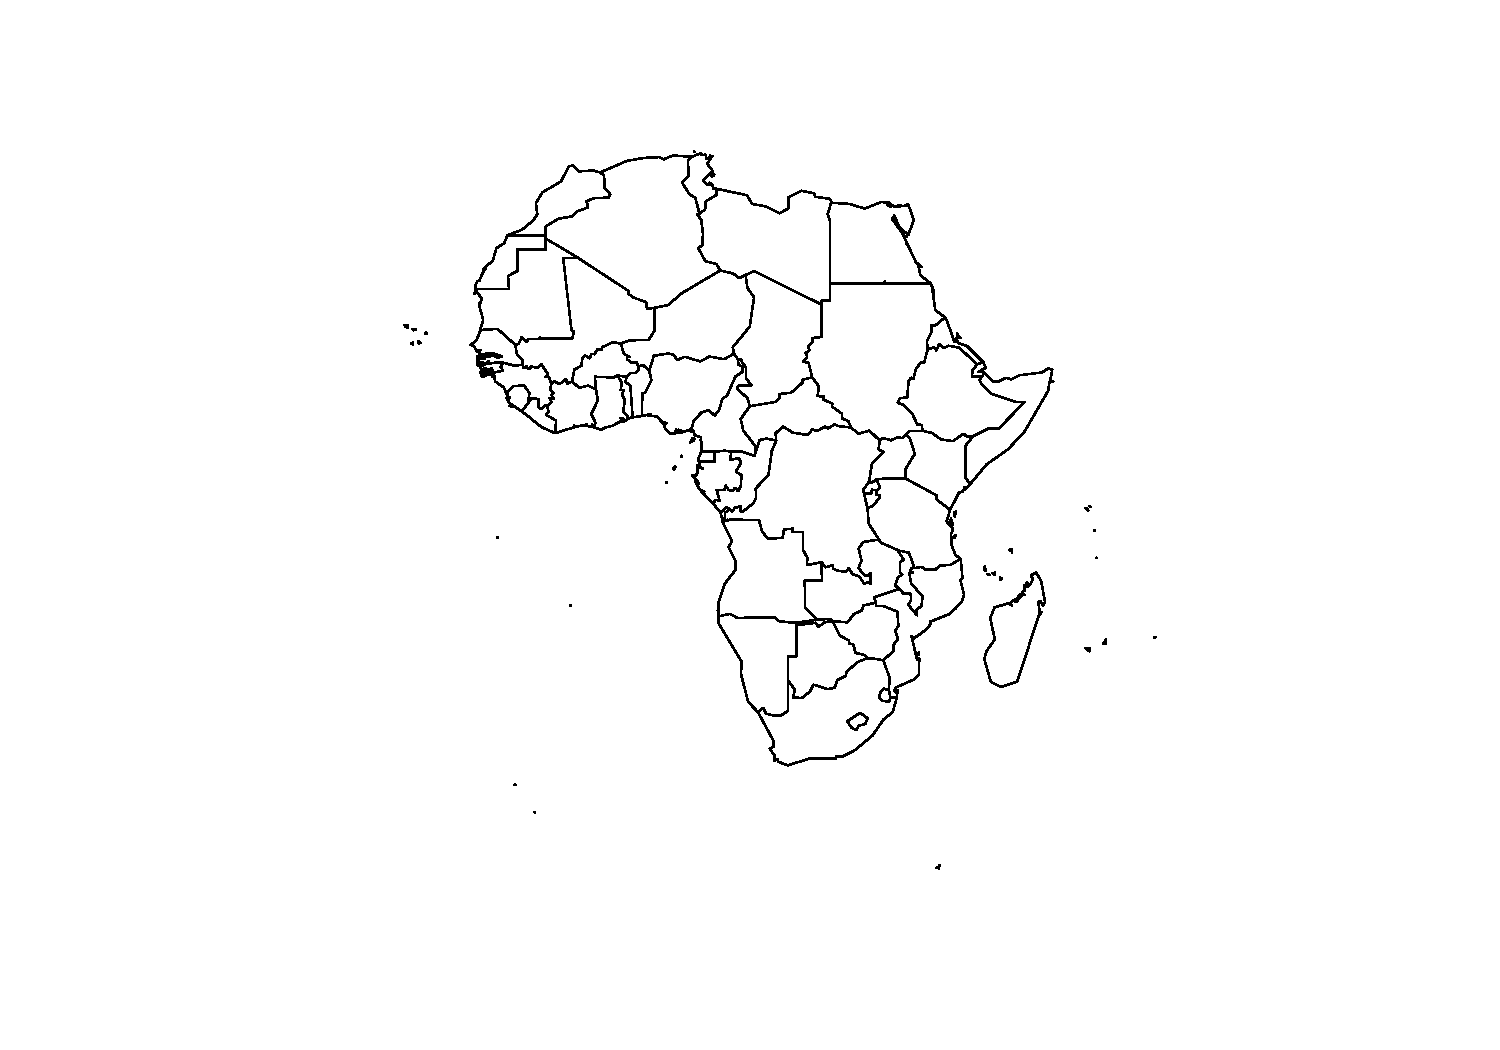
\includegraphics{spdep_files/figure-beamer/unnamed-chunk-1-1.pdf}

\end{frame}

\begin{frame}[fragile]{Das Zentrum eines Polygonzuges}

\begin{Shaded}
\begin{Highlighting}[]
\KeywordTok{library}\NormalTok{(sp)}
\NormalTok{Af <-}\StringTok{ }\KeywordTok{coordinates}\NormalTok{(Africa)}
\KeywordTok{plot}\NormalTok{(Africa)}
\KeywordTok{points}\NormalTok{(}\DataTypeTok{x=}\NormalTok{Af[}\DecValTok{1}\NormalTok{,}\DecValTok{1}\NormalTok{],}\DataTypeTok{y=}\NormalTok{Af[}\DecValTok{1}\NormalTok{,}\DecValTok{2}\NormalTok{],}\DataTypeTok{col=}\StringTok{"red"}\NormalTok{,}\DataTypeTok{pch=}\DecValTok{20}\NormalTok{)}
\end{Highlighting}
\end{Shaded}

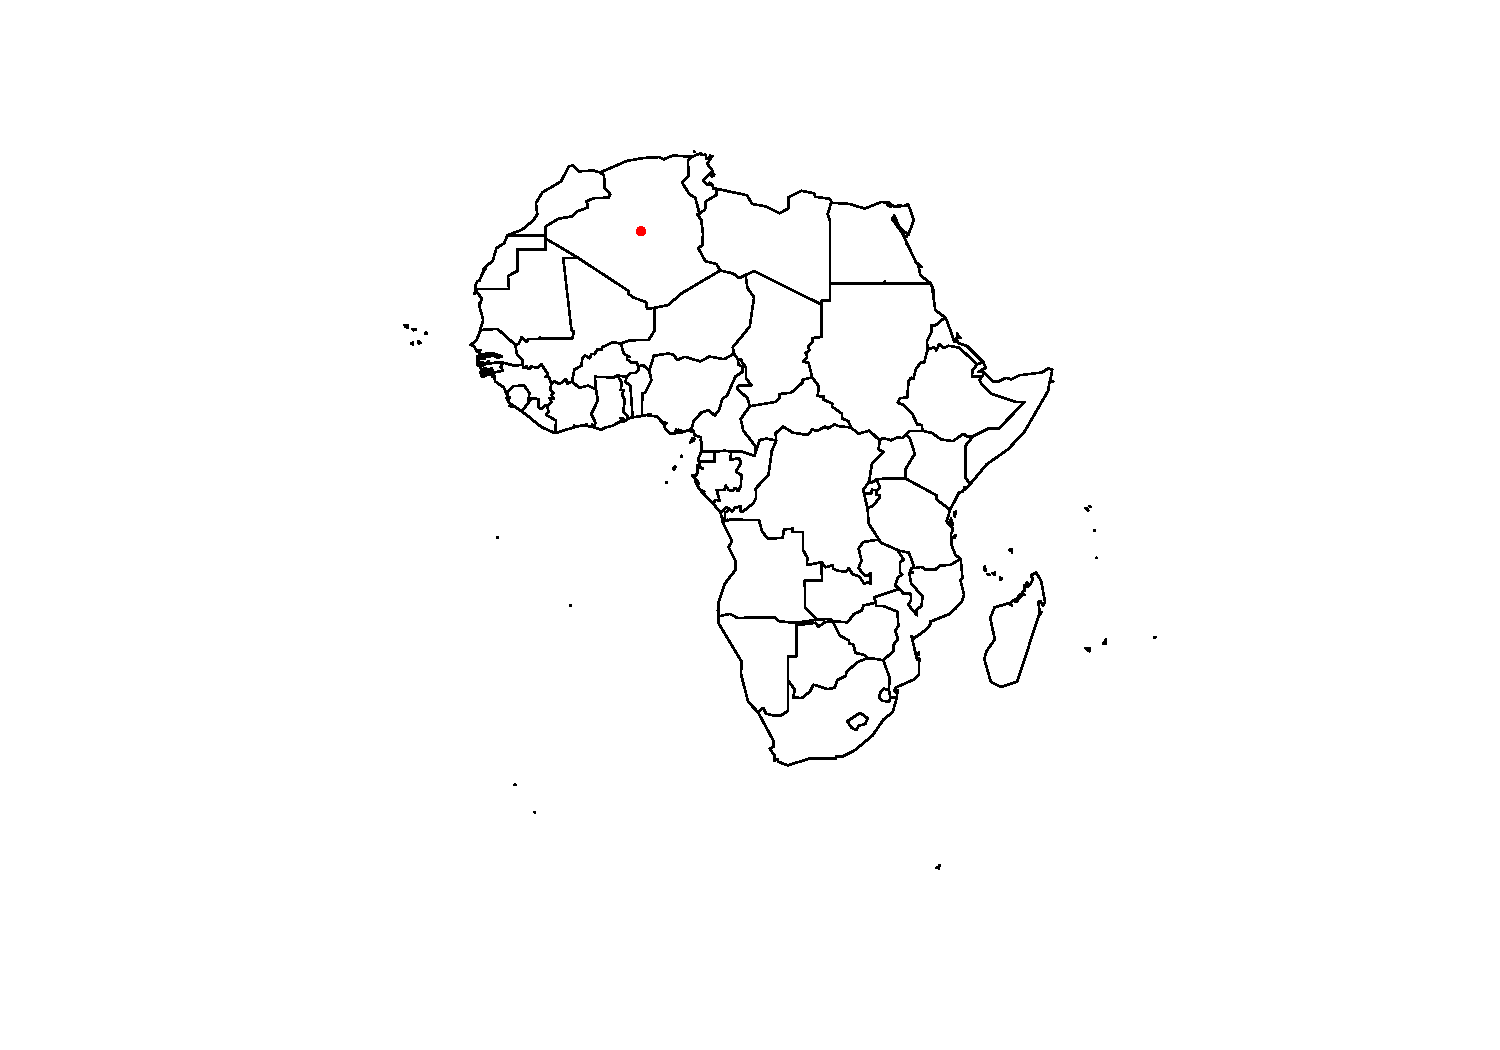
\includegraphics{spdep_files/figure-beamer/unnamed-chunk-2-1.pdf}

\end{frame}

\begin{frame}[fragile]{Die nächsten Nachbarn finden}

\begin{Shaded}
\begin{Highlighting}[]
\KeywordTok{library}\NormalTok{(spdep)}
\NormalTok{Af_nb <-}\StringTok{ }\KeywordTok{tri2nb}\NormalTok{(Af)}
\end{Highlighting}
\end{Shaded}

Die Nachbarn für das erste Land:

\begin{Shaded}
\begin{Highlighting}[]
\NormalTok{Af_nb[}\DecValTok{1}\NormalTok{]}
\end{Highlighting}
\end{Shaded}

\begin{verbatim}
## [[1]]
## [1] 24 26 27 32 48
\end{verbatim}

\end{frame}

\begin{frame}[fragile]{Die Nachbarn finden}

\begin{Shaded}
\begin{Highlighting}[]
\KeywordTok{plot}\NormalTok{(Africa)}
\KeywordTok{plot}\NormalTok{(Africa[}\DecValTok{1}\NormalTok{,],}\DataTypeTok{col=}\StringTok{"red"}\NormalTok{,}\DataTypeTok{add=}\NormalTok{T)}
\KeywordTok{plot}\NormalTok{(Africa[Af_nb[}\DecValTok{1}\NormalTok{][[}\DecValTok{1}\NormalTok{]],],}\DataTypeTok{col=}\StringTok{"orange"}\NormalTok{,}\DataTypeTok{add=}\NormalTok{T)}
\end{Highlighting}
\end{Shaded}

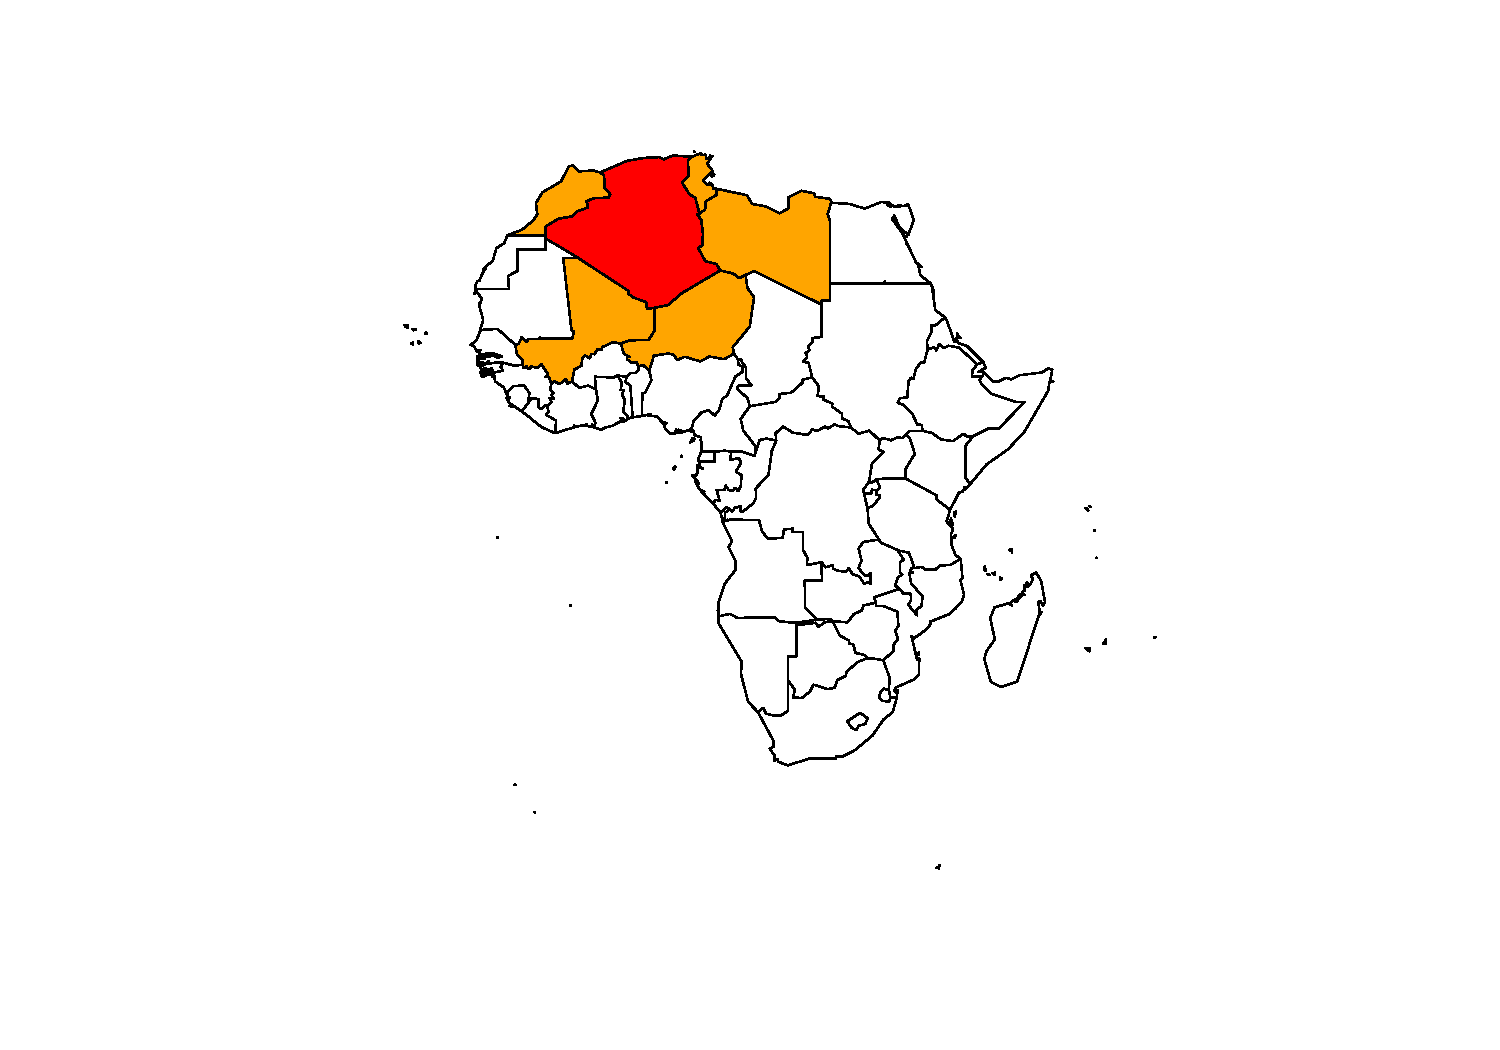
\includegraphics{spdep_files/figure-beamer/unnamed-chunk-5-1.pdf}

\end{frame}

\begin{frame}[fragile]{Die 10 nächsten Nachbarn finden}

\begin{Shaded}
\begin{Highlighting}[]
\NormalTok{IDs <-}\StringTok{ }\KeywordTok{row.names}\NormalTok{(}\KeywordTok{as}\NormalTok{(Africa, }\StringTok{"data.frame"}\NormalTok{))}
\NormalTok{Af10_nb <-}\StringTok{ }\KeywordTok{knn2nb}\NormalTok{(}\KeywordTok{knearneigh}\NormalTok{(Af, }\DataTypeTok{k =} \DecValTok{10}\NormalTok{), }\DataTypeTok{row.names =}\NormalTok{ IDs)}
\KeywordTok{plot}\NormalTok{(Africa)}
\KeywordTok{plot}\NormalTok{(Africa[}\DecValTok{1}\NormalTok{,],}\DataTypeTok{col=}\StringTok{"red"}\NormalTok{,}\DataTypeTok{add=}\NormalTok{T)}
\KeywordTok{plot}\NormalTok{(Africa[Af10_nb[}\DecValTok{1}\NormalTok{][[}\DecValTok{1}\NormalTok{]],],}\DataTypeTok{col=}\StringTok{"orange"}\NormalTok{,}\DataTypeTok{add=}\NormalTok{T)}
\end{Highlighting}
\end{Shaded}

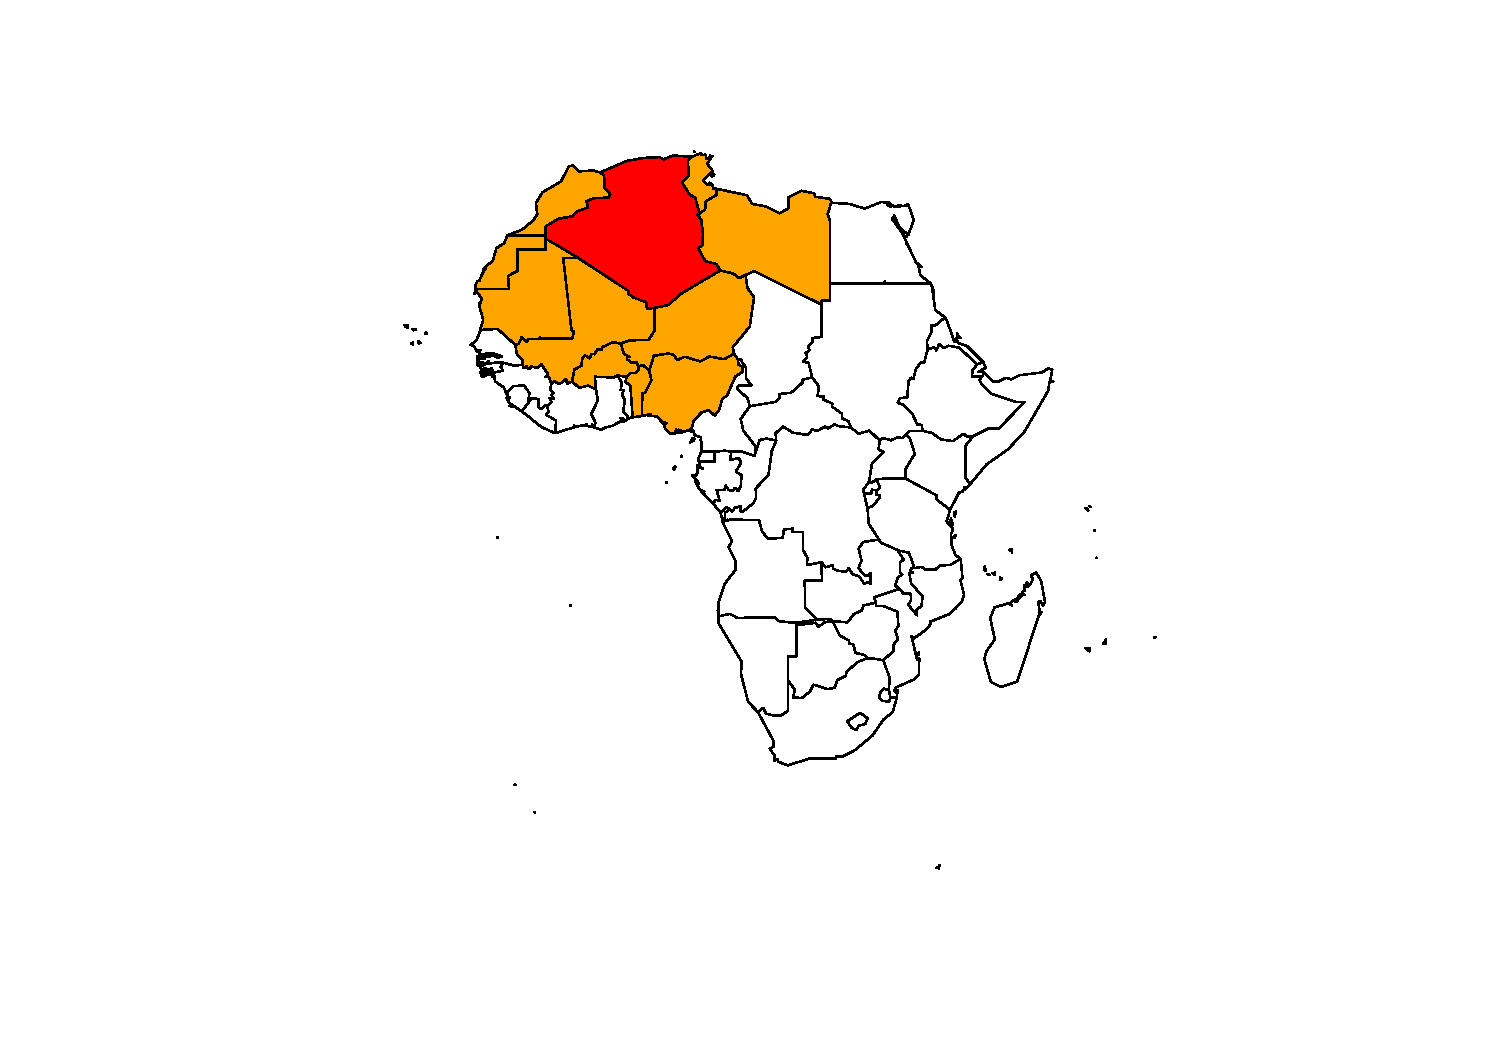
\includegraphics{spdep_files/figure-beamer/unnamed-chunk-6-1.pdf}

\end{frame}

\begin{frame}[fragile]{Die Distanz berechnen}

\begin{Shaded}
\begin{Highlighting}[]
\NormalTok{Af <-}\StringTok{ }\KeywordTok{coordinates}\NormalTok{(Africa) }\CommentTok{# get centroid}
\KeywordTok{library}\NormalTok{(raster)}
\KeywordTok{pointDistance}\NormalTok{(Af[}\DecValTok{1}\OperatorTok{:}\DecValTok{4}\NormalTok{,], }\DataTypeTok{lonlat=}\OtherTok{TRUE}\NormalTok{) }\CommentTok{# compute distance}
\end{Highlighting}
\end{Shaded}

\begin{verbatim}
##         [,1]    [,2]    [,3] [,4]
## [1,]       0      NA      NA   NA
## [2,] 4763231       0      NA   NA
## [3,] 2055609 2954497       0   NA
## [4,] 3484053 1295173 1839191    0
\end{verbatim}

\end{frame}

\begin{frame}[fragile]{Berechnen/zeichnen einer Distanzmatrix}

\begin{Shaded}
\begin{Highlighting}[]
\NormalTok{Dist_Af <-}\StringTok{ }\KeywordTok{pointDistance}\NormalTok{(Af, }\DataTypeTok{lonlat=}\OtherTok{TRUE}\NormalTok{)}
\NormalTok{Af_color <-}\StringTok{ }\NormalTok{Dist_Af[,}\DecValTok{1}\NormalTok{]}
\NormalTok{Af_color <-}\StringTok{ }\NormalTok{Af_color}\OperatorTok{/}\KeywordTok{max}\NormalTok{(Af_color)}
\NormalTok{Af_color <-}\StringTok{ }\KeywordTok{rgb}\NormalTok{(Af_color,}\DecValTok{0}\NormalTok{,}\DecValTok{0}\NormalTok{)}
\KeywordTok{plot}\NormalTok{(Africa,}\DataTypeTok{col=}\NormalTok{Af_color)}
\end{Highlighting}
\end{Shaded}

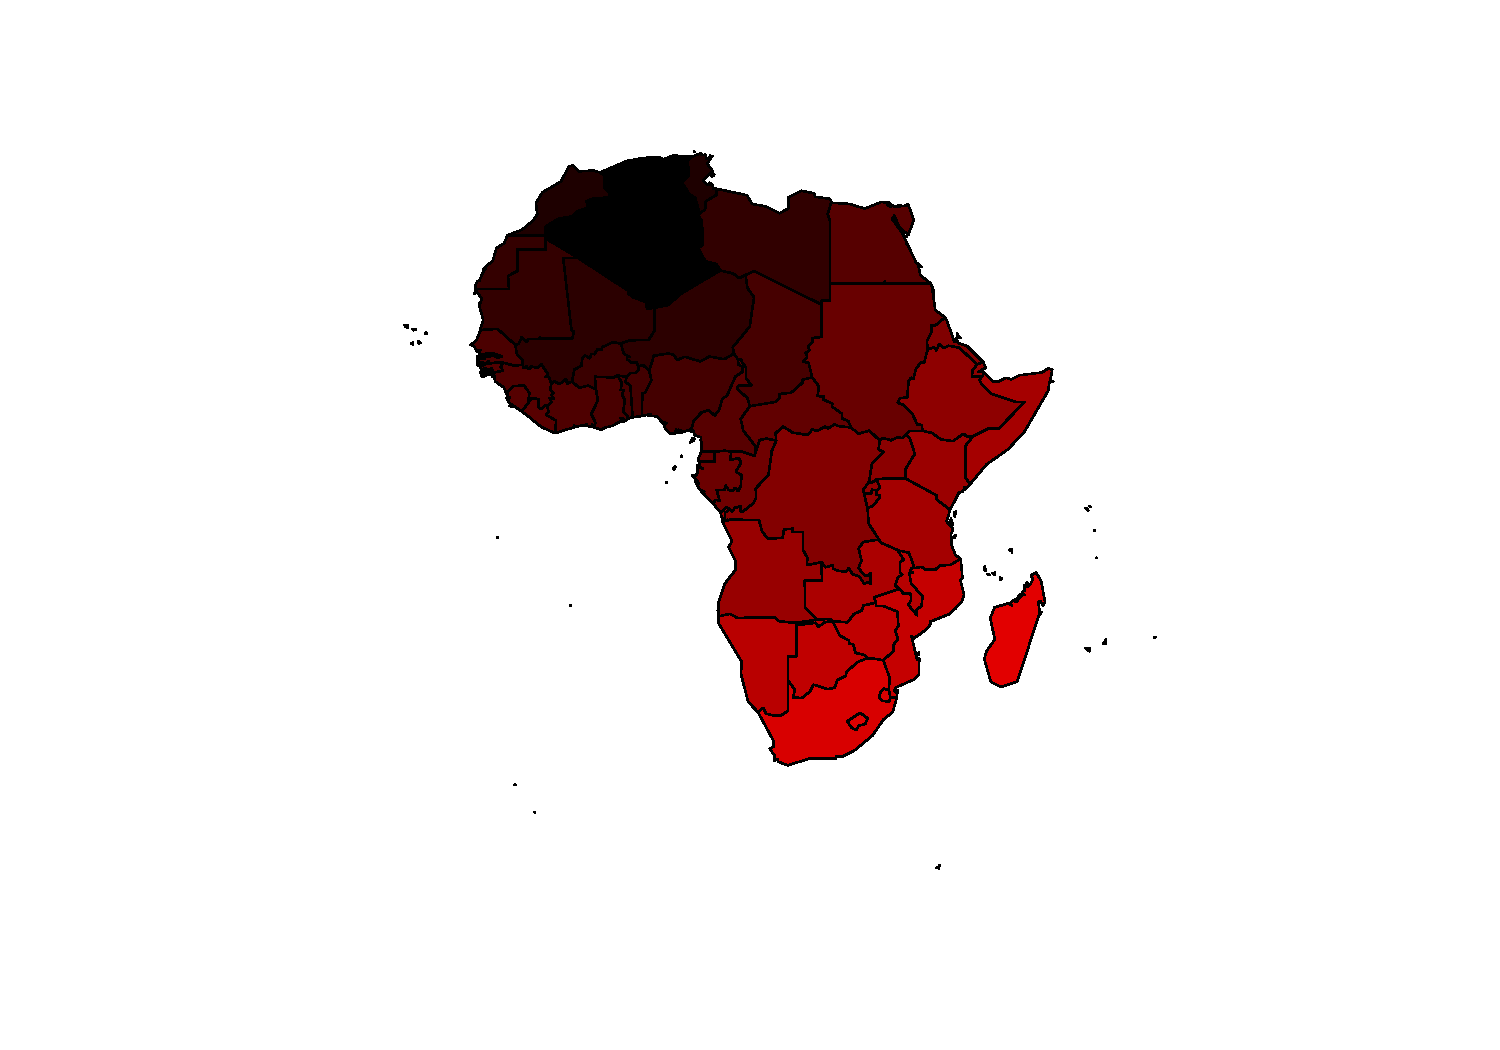
\includegraphics{spdep_files/figure-beamer/Africa Distance-1.pdf}

\end{frame}

\begin{frame}[fragile]{Aufgabe}

\begin{Shaded}
\begin{Highlighting}[]
\KeywordTok{library}\NormalTok{(sf)}
\end{Highlighting}
\end{Shaded}

\begin{verbatim}
## Linking to GEOS 3.6.1, GDAL 2.2.3, proj.4 4.9.3
\end{verbatim}

\begin{Shaded}
\begin{Highlighting}[]
\NormalTok{lnd <-}\StringTok{ }\KeywordTok{read_sf}\NormalTok{(}\StringTok{"../data/london_sport.shp"}\NormalTok{)}
\end{Highlighting}
\end{Shaded}

\end{frame}

\begin{frame}{Links}

\begin{itemize}
\tightlist
\item
  \href{https://procomun.wordpress.com/2011/06/17/raster-cmsaf-and-solar/}{Raster,
  CMSAF and solaR}
\end{itemize}

\url{https://procomun.wordpress.com/2011/06/17/raster-cmsaf-and-solar/}

\begin{itemize}
\tightlist
\item
  \href{https://johnbaumgartner.wordpress.com/2012/07/26/getting-rasters-into-shape-from-r/}{Getting
  rasters into shape from R}
\end{itemize}

\url{https://johnbaumgartner.wordpress.com/2012/07/26/getting-rasters-into-shape-from-r/}

\end{frame}

\end{document}
